%%%%%%%%%%%%%%%%%%%%%%%%%%%%%%%%%%%%%%%%%%%%%%%%%%%
%
%  New template code for TAMU Theses and Dissertations starting Fall 2016.  
%
%
%  Author: Sean Zachary Roberson
%  Version 3.17.09
%  Last Updated: 9/21/2017
%
%%%%%%%%%%%%%%%%%%%%%%%%%%%%%%%%%%%%%%%%%%%%%%%%%%%
%%%%%%%%%%%%%%%%%%%%%%%%%%%%%%%%%%%%%%%%%%%%%%%%%%%%%%%%%%%%%%%%%%%%%%
%%                           SECTION V
%%%%%%%%%%%%%%%%%%%%%%%%%%%%%%%%%%%%%%%%%%%%%%%%%%%%%%%%%%%%%%%%%%%%%



\chapter{ANALYSIS \label{cha:analysis}}

%Here an overview of the strategy, decribe signal generaly, what does it look like. Then the background, how to discriminate s/b to motivate following subsections.
This study presents the search for a heavy boson resonance, a Z', decaying into two $b$ quarks. Such particle arises from the fusion of two $b$ quarks which are in turn a result of gluon splitting. The final state then, consists of four $b$ quarks, two of them being direct decay products of the resonance and two additional associated quarks from the initial gluon splitting.

The search for a Z' is motivated by the anomalies in B-meson decays reported by the Belle and LHCb experiments. Similar searches for a Z' boson have been performed previously (e.g.) and a similar analysis looking in to a di-muon + jets final states is currently being carried out in parallel\cite{PhysRevD.97.075035}.

The search is performed using a data sample of proton-proton collisions at a center-of-mass energy of 13 TeV collected by the CMS experiment in 2016 and corresponding to an integrated luminosity of 35.9$fb^{-1}$. Data for this analysis was collected using a HLT that uses multi-jet and $b$-tagging requirements as described in Section \ref{sec:trigger}.

The Z' decay is reconstructed offline from its decay products by considering the two leading jets in $p_{T}$ in the event. The discriminant variable of choice is the di-jet invariant mass of PF jets clustered using the anti-$k_{T}$ algorithm with a size parameter of 0.4 and which are tagged by using the DeepCSV algorithm as being consistent with a $b$-quark hadron. 

As one could expect from an all-hadronic final state search, any signal for the process of interest would be buried under an immense background of multi-jet events produced by QCD interactions. For this purpose, a signal region is identified by means of a specific $b$-tagging selection on the 4 leading jets on $p_{T}$ and an offline trigger as described in Sections \ref{sec:selection} and \ref{sec:trigger}. The background control regions are orthogonal to the SR in terms of the trigger and $b$-tagging selection used for the SR. Then, a data-driven method is used to estimate the background contribution due to the poorly-understood multi-jet QCD backgrounds. 

Once the contribution from uncertainties is well understood and the data-driven method is validated, the SR will be unblinded and the limits on the production cross section are calculated.

\section{Data and Monte Carlo Samples \label{sec:datasets}}
\subsection{Data}
As mentioned previously, this analysis makes use of the full 2016 CMS dataset of 13 TeV data. Table \ref{tab:dataSamples} shows the data samples used for this analysis, which correspond to a total of 35.9$fb^{-1}$ of data. 

\begin{table}[hbtp]\footnotesize
\centering
\begin{tabular}{l l l}
\hline
 Dataset & Run Range & Integrated Luminosity \\
\hline
/BTagCSV/Run2016B-07Aug17-v*/AOD & 272007-275376 & 5.8 \\
/BTagCSV/Run2016C-07Aug17-v1/AOD & 275657-276283 & 2.5 \\
/BTagCSV/Run2016D-07Aug17-v1/AOD & 276315-276811 & 4.3 \\
/BTagCSV/Run2016E-07Aug17-v1/AOD & 276831-277420 & 4.1 \\
/BTagCSV/Run2016F-07Aug17-v1/AOD & 277772-278808 & 3.1 \\
/BTagCSV/Run2016G-07Aug17-v1/AOD & 278820-280385 & 7.5 \\
/BTagCSV/Run2016H-07Aug17-v1/AOD & 280919-284044 & 8.5 \\
{\bf Total BTagCSV} & {\bf 272007--284044} & {\bf 35.9} \\
\hline
/SingleMu/Run2016B-07Aug17-v*/AOD & 272007-275376 & 5.8 \\
/SingleMu/Run2016C-07Aug17-v1/AOD & 275657-276283 & 2.5 \\
/SingleMu/Run2016D-07Aug17-v1/AOD & 276315-276811 & 4.3 \\
/SingleMu/Run2016E-07Aug17-v1/AOD & 276831-277420 & 4.1 \\
/SingleMu/Run2016F-07Aug17-v1/AOD & 277772-278808 & 3.1 \\
/SingleMu/Run2016G-07Aug17-v1/AOD & 278820-280385 & 7.5 \\
/SingleMu/Run2016H-07Aug17-v1/AOD & 280919-284044 & 8.5 \\
{\bf Total SingleMu} & {\bf 272007--284044} & {\bf 35.9} \\
\hline
\end{tabular}
\caption{The datasets analyzed for this analysis.}
\label{tab:dataSamples}
\end{table}

 Data is processed in the CMSSW$\_$9$\_$4$\_$9 framework to yield \textit{n-tuples} which include a subset of the information contained in the official CMS datasets. These smaller datasets were analyzed using privately created analysis software.

\subsection{Monte Carlo}

This analysis makes use of MC simulation to study the background processes which have similar states to that of the signal. These simulations are also used to optimize the event selection and to cross-check the data-based background estimations. Table \ref{tab:bkgSamples} lists all of the MC samples for the considered SM background processes, which are centrally produced by the CMS collaboration.


\begin{sidewaystable}[hbtp]\footnotesize
	\centering
	\begin{tabular}{l p{0.65\textwidth} l}
		\hline
		\multicolumn{3}{c}{Background Processes} \\
		\hline
		Process & Dataset Name & Cross Section [pb] \\
		\hline
		QCD\_HT50to100 & QCD\_HT50to100\_TuneCUETP8M1\_13TeV-madgraphMLM-pythia8 & 246300000.0 \\
		QCD\_HT100to200 & QCD\_HT100to200\_TuneCUETP8M1\_13TeV-madgraphMLM-pythia8 & 28060000.0\\
		QCD\_HT200to300 & QCD\_HT200to300\_TuneCUETP8M1\_13TeV-madgraphMLM-pythia8 & 1710000.0 \\
		QCD\_HT300to500 & QCD\_HT300to500\_TuneCUETP8M1\_13TeV-madgraphMLM-pythia8 & 347500.0\\ 	
		QCD\_HT500to700 & QCD\_HT500to700\_TuneCUETP8M1\_13TeV-madgraphMLM-pythia8 & 32060.0\\ 
		QCD\_HT700to1000 & QCD\_HT700to1000\_TuneCUETP8M1\_13TeV-madgraphMLM-pythia8 & 6829.0\\
		QCD\_HT1000to1500 & QCD\_HT1000to1500\_TuneCUETP8M1\_13TeV-madgraphMLM-pythia8 & 1207.0\\	
		QCD\_HT1500to2000 & QCD\_HT1500to2000\_TuneCUETP8M1\_13TeV-madgraphMLM-pythia8 & 120.0\\ 
		QCD\_HT2000toInf & QCD\_HT2000toInf\_TuneCUETP8M1\_13TeV-madgraphMLM-pythia8 & 25.25\\ 
		TTJets & TTJets\_TuneCUETP8M2T4\_13TeV-amcatnloFXFX-pythia8 & 831.76\\
		\hline
	\end{tabular}
	\caption{List of background MC datasets and cross sections used in the analysis. Every dataset name is followed by /RunIISummer16MiniAODv2-PUMoriond17\_80X\_mcRun2\_asymptotic\_2016\_TrancheIV\_v6-v1/MINIAODSIM.}
	\label{tab:bkgSamples}
\end{sidewaystable}

The signal sample kinematics and yields are also taken from MC, but a dataset was produced privately and specifically for this analysis. The MC signal events are simulated to leading order (LO) in QCD precision. Different samples are generated for $m_{X}$ ranging from 350 to 950 GeV. Also, the model attempts to exclude a phase space spanned by $g_{b}$, $g_{\mu}$, $g_{\tau}$ and $\delta_{bs}$ and therefore different values for $\delta_{bs}$ were considered ranging from 0.0 to 1.0 in steps of 0.25. The coupling parameter $g_{b}$ was set to 0.1 and the rest of the parameters to 0.0.  The MADGRAPH5 v4.2.4 event generator was used with the NNPDF3.0 leading order PDFs taken from the LHAPDF 6.2.1 PDF set. The showering and hadronization of partons was simulated with PYTHIA 8 with the CUETP8M1 NNPDF23LO tune. Finally, the hadronization and reconstruction was performed by using the CMSSW release 8$\_$0$\_$26.

MC background events were generated using the leading-order matrix element generator MADGRAPH5 v4.2.4. Parton shower and hadronization are included using PYTHIA 6.4.26, and the matrix element is matched to the parton shower using the MLM scheme. The Z2* tune is used to describe the underlying event. This tune is identical to the Z1 tune, but uses the CTEQ6L PDFs.

All generated events are processed through a simulation of the CMS apparatus based on GEANT4. Additional proton-proton interactions within a bunch crossing (pileup) are added to the simulation, with a frequency distribution chosen to match that observed in data. During this data-taking period the mean number of interactions per bunch crossing is 25.

\subsubsection{Multi-jet QCD Background}
It is well known that the QCD process is difficult to model to the desired level of accuracy. Additionally, the event selection in the analysis requires four jets, which vastly reduces the number of QCD MC events that pass the selection criteria and therefore, when using the MC samples we are left with a statistically limited sample that is almost useless for describing this background.

Rather than relying on MC for the QCD background sample, a data-driven method to estimate the contribution from background in the signal region will be used. This method is explained in detail in Section \ref{sec:datadriven}.
%\subsubsection{Data to MC Comparison}

\section{Object Selection}

As described in Chapter 4, CMS provides every user a list of reconstructed objects (i.e. jets, electrons, etc.) which may be used. However, these reconstruction algorithms are intentionally generic so that the objects they return are applicable to a wide array of physics analyses. Specific groups within CMS called physics object groups (POGs) are responsible for developing object quality criteria which must be implemented by each analysis to prevent fake or poorly reconstructed objects. This section will discuss the object selection criteria to identify jets, which all meet or exceed the object requirements as set by the relevant POGs. Only events which contain objects of the right quality and multiplicities will be used in this analysis.

Jets used for this analysis must meet the Tight Jet ID criteria as described in Section \ref{sec:jets}. Moreover, selected jets must have a $p_{T}$ > 30 GeV and $|\eta|$ < 2.6. Since b-jet identification plays a key role in identifying the signal,the four leading jets on the event are required to be b-tagged.

\section{Data and MC Corrections}

Despite the efforts to make sure the MC simulation models data properly, there can still exist discrpeancies between the observed data and simulation. OFten this occurs because the exact data taking conditions are not known in advance, like the pileup conditions during the actual run of the experiment. In other cases, this discrepancies arise from the precision of the physics generators, which might not be enough to model data accurately. A significant part of the physics of hadronization is still unkown and hard physics process can often be computed up to NLO precision. Data on the other hand, contains all hadronization effects and all orders of precision. 

In Sections and I have already discussed some object-specific corrections like jet energy corrections and resolution. For other discrepancies, it is often necessary to reweight the full event rather than a specific object and they are specific to the analysis. In the following sections, an attempt to explain some of these corrections is made.

\subsection{JEC and Residuals}
The details of the factorized approach adopted by CMS for jet energy calibration were discussed in Section. The final step in this chain are the residual corrections applied to data, to account for data to MC differences.

To address residual differences between data and simulation, the additional scale factors are evaluated after correcting jets for pileup and simulated particle response. The basic idea is to exploit the transverse momentum balance between the jet to be calibrated and the reference object.

\subsection{JER Smearing}
The jet $p_{T}$ resolution is relatively poor compared to the resolution of many other physics objects, and the biases caused by jet resolution smearing can be important for steeply falling spectra and for resonance decays like the Z'. At CMS, the particle-level JER is determined from MC simulation and then a data/MC scale factor is obtained from data-based methods. Note that JECs are applied as described in Section before deriving JER.

A detailed description of the Methods can be found at \cite{jes_jer} but strictly speaking one could say that the measurement of JER is an extension of the methods used for measuring JES, but instead of looking at the mean of the response distribution, we are interested in its width.

\subsection{Pileup Re-weighting}
Up to this point, pileup has been described as additional proton-proton interactions within an event, besides the interaction that produced the physics objects we are interested in studying, but there are several and other properties of pileup which are worth noting. First, pileup is related to additional objects (tracks or energy) which might be found in the same bunch crossing as the event under study. In reality, there are two different kinds of pileup. There is indeed pileup which comes from additional proton-proton interactions within the same bunch crossing, known as "in-time" pileup, but there is also energy from pileup added to objects becaus eit was left in the sub-detectors from bunch crossing before or after the current one. This is known as "out-of-time" pileup and is largely due to the fact that the integration window of the sub-detectors can be larger than 25 ns. 

Second, the true number of proton-proton interactions within an event, $\mu$ is related to the instantaneous luminosity, which can vary within any given data taking period and even within a luminosity section (LS). As a benchmark, the average number of proton-proton interactions per bunch crossing in 2016 was 23.

Finally, pileup can affect the reconstruction efficiency and even the observed kinematics of all the objects used in the analysis and therefore it is of vital importance that the pileup distribution in MC follows that of data as close as possible. 

Since the MC samples used in CMS are usually produced before the data was taken, the actual pileup conditions were unknown during the generation process. Thus, MC was generated assuming specific conditions that might not match data that well. A broad distribution of $\mu$ values, the number of mini-bias pileup events overlaid on the hard scatter event, is generally chosen so as to cover all pileup conditions which mught be ecperienced over the course of a data taking period. Unsurpsisingly, the anticipated $\mu$ distribution rarely matches the observed one in data and thus the MC must be reweighted such that the $\mu$ distributions match.
 %reference 167 in Alexx' thesis



\begin{figure}
	\centering
	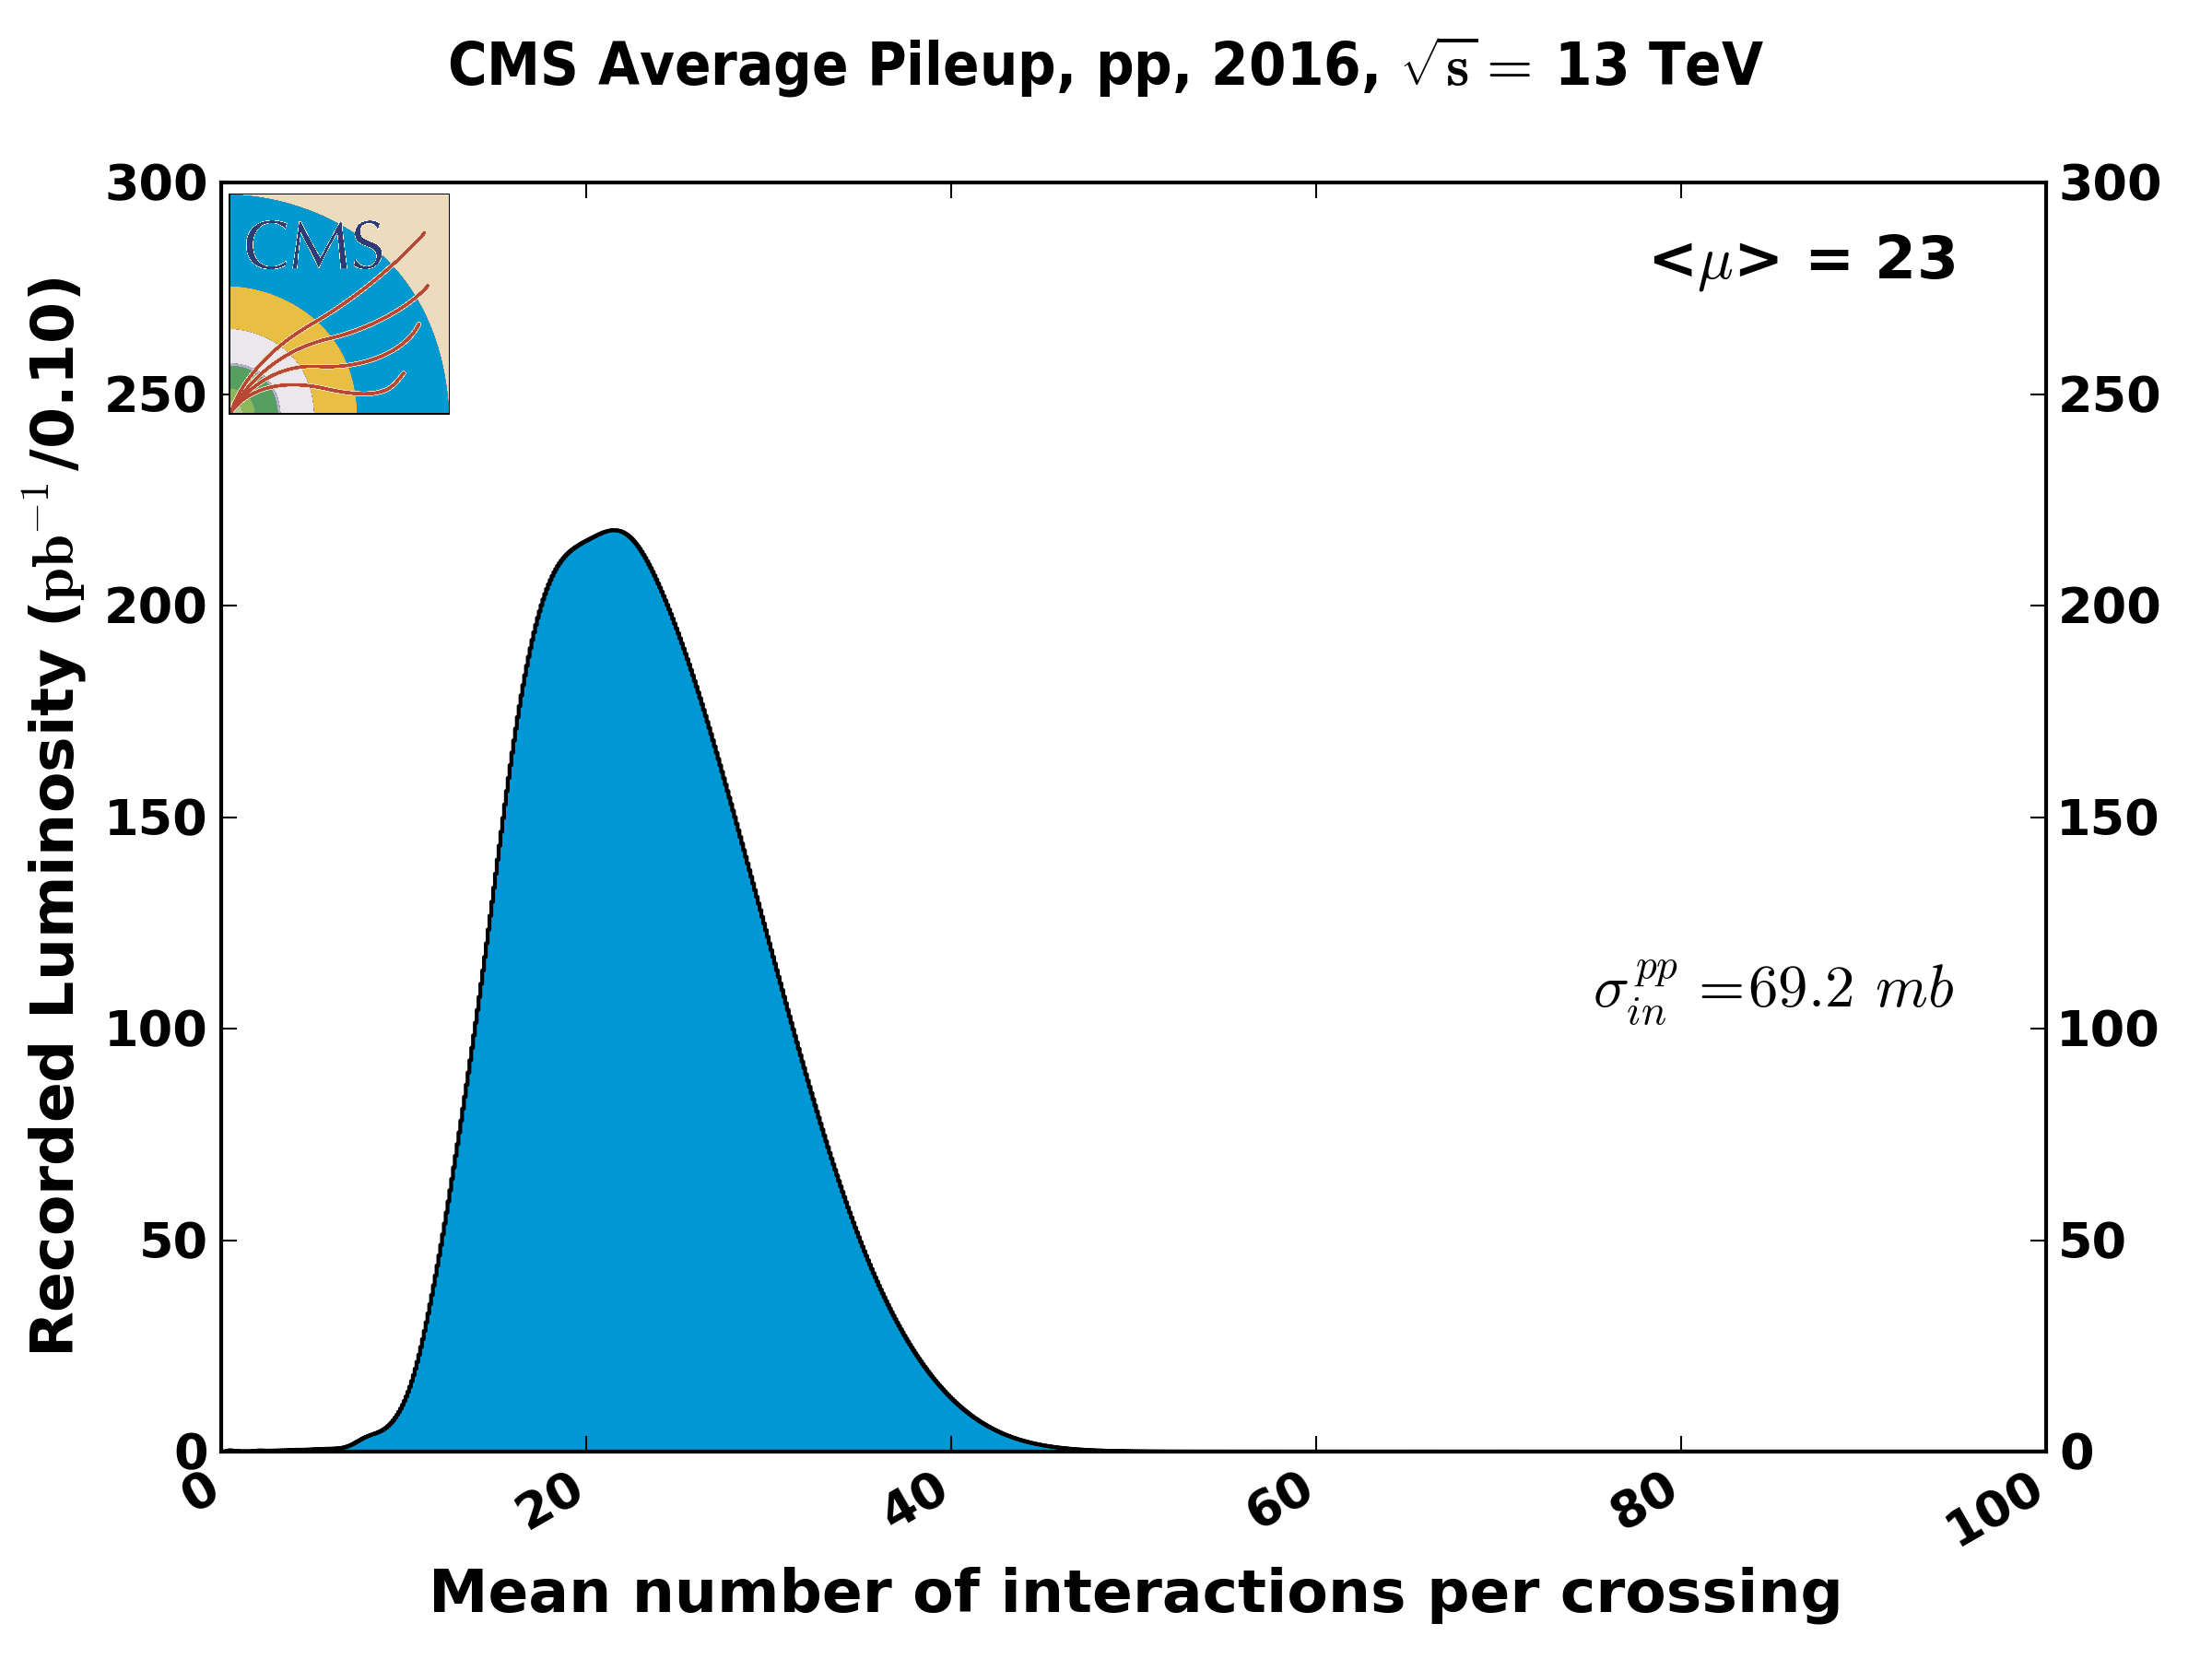
\includegraphics[width=0.45\textwidth]{figures/pileup_pp_2016_69200.png}
	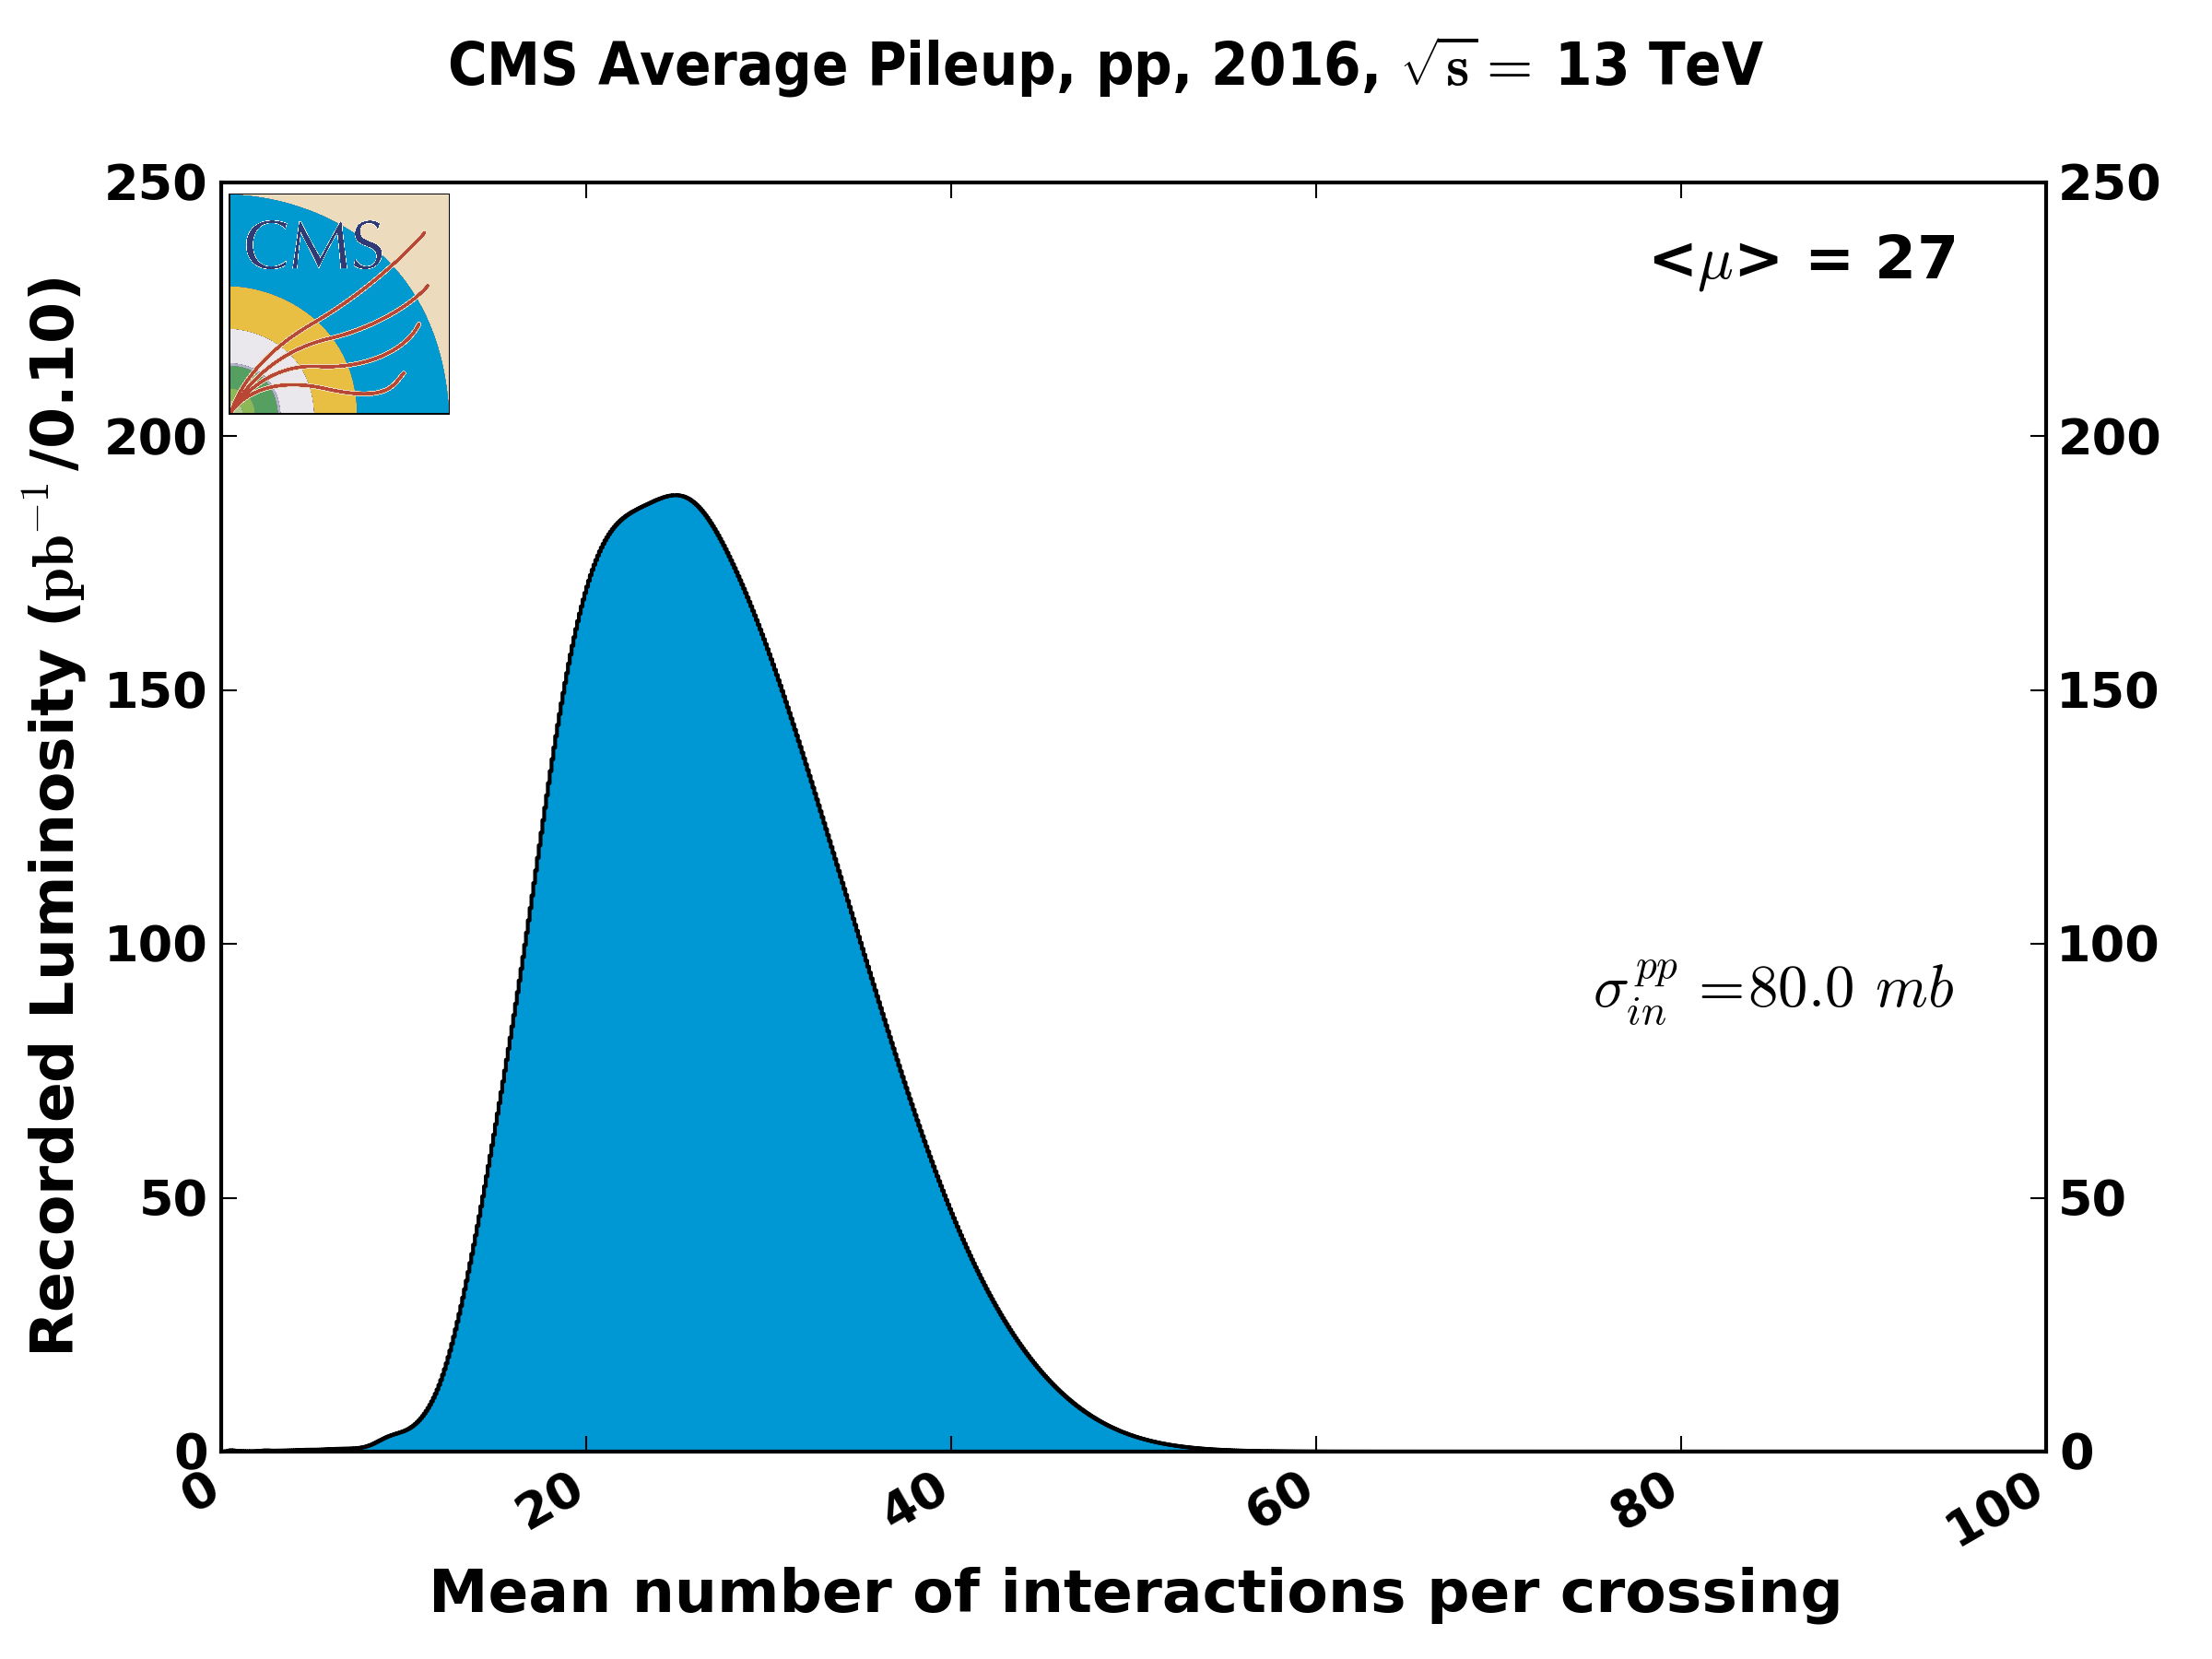
\includegraphics[width=0.45\textwidth]{figures/pileup_pp_2016_80000.png}
	\singlespace
	\caption{Mean number of interactions per bunch crossing for the 2016 proton-proton run at $\sqrt{s}$=13 TeV. The two plots shown here use the same data but different values for the minimum bias cross section were assumed. The left plot uses the "CMS recommended" value of 69.2 mb, which is determined by finding the best agreement with data and is recommended for CMS analyses. The right plot uses the "LHC standard" value of 80 mb, which is taken from the theoretical prediction from Pythia and should be used to compare to other LHC experiments\cite{cmslumitwiki}}.
	\label{fig:cmspu}
	
\end{figure}

To generate a histogram for the average number of interactions per bunch crossing coming from data we make use of the approved pileupCalc tool provided by CMS. This tool takes as input the total inelastic cross section $\sigma_{inelastic}$ = 69.2, a "pileup file" in JSON format (provided centrally by CMS for every data taking period) with every run number and luminosity section matched to a given average instantaneous luminosity and integrated luminosity for that given luminosity section, and another JSON formatted file with the run numbers and luminosity section used in the given analysis. In order to account for the prescaling in the trigger path used in the analysis, the analysis json file was modified.

First, the delivered and recorded luminosity per lumi section for the analysis trigger paths we are calculated by using the brilcalc tool. This step generates a file that is the input to the pileupReCalcl$\_$HLTpaths.py script which generates a new version of the pileup file where weights are applied to each lumi section in the pileup distribution where the recorded luminosity is smaller than nominal due to trigger prescales. 

The per event weights as a function of $\mu$ are created by dividing the normalized distribution from data by the normalized MC based distribution. The weights are then applied to each MC event by looking up the weight for the mean number of pileup interactions used to generate that specific event.
%\cite 168 in Alexx' thesis

The distributions of pileup interactions in MC and data as well as the corresponding pileup weight can be seen in Figure for MC generated signal for a Z' with a mass of 500 GeV.

\subsection{CSV Reweighting}

In Section, a criterion for tagging a jet as being produced by a $b$ quark and the used of the CSV discriminant was introduced. The derivation of this discriminant is described in .%cite Alexx' 137,138

This analysis relies heavily in the ability to identify $b$ jets, so it is absolutely crucial that it behave the same in both data and MC and accurately describe the rate of observing a $b$ jet. In ref 169 is noted that the tagging efficiency in data is not the same as that in MC, so a correction to the CSV discriminant must be made. The corrections described there correct both the rate of observing a jet in MC with a CSV value above a given threshold as well as the general shape of the CSV distribution. IF at the end of the procedure the shape of the data and MC distributions agree, then they will also properly assess the rate of events passing a given CSV threshold.

The method is based on calculating a scale factor for both heavy and light flavor quarks which is parameterized by the CSV value, jet $p_{T}$, and, in the case of light flavor quarks, jet $\eta$. We first retrieve the truth level jet flavor in order to determine the correct category: $b$ jet, $c$ jet, or light flavor (anything else). The $c$ jets are given a flat scale factor of 1, meaning that there is no need to correct the CSV value for this flavor. The $b$ jet scale factors are divided into five $p_{T}$ bins of $p_{T}$ < 40 GeV, 40 GeV <  $p_{T}$ < 60 GeV, 60 GeV <  $p_{T}$ 100 GeV, 100 GeV <  $p_{T}$ 160 GeV, $p_{T}$ > 160 GeV. The light flavor scale factors are divided into nly three $p_{T}$ bins of $p_{T}$ < 40 GeV, 40 GeV <  $p_{T}$ < 60 GeV, but are also divided in $\eta$ bins of |$\eta$| < 0.8, 0.8 $\geq |\eta|$ < 1.6, and 1.6 $\geq |\eta|$ < 2.4. An individual scale factor is retrieved for each jet, which is then combined as in Equation in order to create an event weight.

\begin{equation}
SF_{total} = \prod_{i}^{N_{jets}}SF_{jet_{i}} = SF_{jet_{1}}\cdot SF_{jet_{2}}\cdot ... 
\end{equation}
The CSV value for each jet is unchanged, but the event is weighted by $SF_{total}$.

\section{Trigger \label{sec:trigger}}

Events used in this analysis are selected by trigger algorithms that save events with a large amount of hadronic activity. The L1 seeds for these triggers either select events with a large scalar sum of jet transverse momentum ($H_{T}$) or that contain a jet with a high $p_{T}$. The HLT algorithm then places requirements on either the event $H_{T}$, jet $p_{T}$, or jet tagging. 

The final state characterized by 4 b-jets is particularly challenging to trigger on with the usual multi-trigger paths due to the immense rate of QCD multi-jet events. In order to have low thresholds for jet $p_{T}$ appropriate for the analysis and an acceptable rate, a trigger exploiting the b-tag information at the HLT level has been chosen.

The use of b-tagging at trigger level also reduces the multi-jet contribution to the selected data sample. The paths used are DoubleJet90$\_$Double30$\_$TripleCSV087 and Quad45$\_$TripleCSV087 and they are described below. 

Schematically, these HLT paths seed on events that contain basically high L1 HT. In order to increase the L1 trigger efficiency, other multi-jet seeds have been used in logic OR. Then, the HLT paths select events with four HLT anti-kT4 jets above four optimized $p_{T}$ thresholds, and then requires a minimum HLT b-tagging value for three jets with full regional HLT tracking information. 

The HLT path structure can be summarized as:

\textbf{DoubleJet90$\_$Double30$\_$TripleBTagCSV$\_$p087:}
\begin{itemize}
	\item L1$\_$TripleJet$\_$84$\_$68$\_$48$\_$VBF OR L1$\_$TripleJet$\_$88$\_$72$\_$56$\_$VBF OR\\ L1$\_$TripleJet$\_$92$\_$76$\_$64$\_$VBF OR L1$\_$HTT280 OR L1$\_$HTT300 OR L1$\_$HTT320 OR L1$\_$SingleJet170 OR L1$\_$SingleJet180 OR L1$\_$SingleJet200 OR L1$\_$DoubleJetC100 OR L1$\_$DoubleJetC112 OR L1$\_$DoubleJetC120
	\item Reconstruct anti-$k_{T}$ 0.4 L1FastJet corrected Calo-jets
	\begin{itemize}
		\item 2 jets with $|\eta|$ < 2.6 and $p_{T}$ > 90 GeV
		\item 4 jets with $|\eta|$ < 2.6 and $p_{T}$ > 30 GeV		
	\end{itemize}
	\item Fast Primary Vertex Reconstruction
	\item Online CSV computation
	\begin{itemize}
		\item 3 Calo-jets with CSV>0.87
	\end{itemize}
	\item PF reconstruction sequence
	\begin{itemize}
		\item 2 PF jets with $|\eta|$ < 2.6 and $p_{T}$ > 90 GeV
		\item 4 PF jets with $|\eta|$ < 2.6 and $p_{T}$ > 30 GeV		
	\end{itemize}
\end{itemize}

\textbf{QuadJet45$\_$TripleBTagCSV$\_$p087:}
\begin{itemize}
	\item L1$\_$QuadJetC50 OR L1$\_$QuadJetC60 OR L1$\_$HTT280 OR L1$\_$HTT300 OR L1$\_$HTT320 OR L1$\_$TripleJet$\_$84$\_$68$\_$48$\_$VBF OR L1$\_$TripleJet$\_$88$\_$72$\_$56$\_$VBF OR L1$\_$TripleJet$\_$92$\_$76$\_$64$\_$VBF
	\item Reconstruct anti-$k_{T}$ 0.4 L1FastJet corrected Calo-jets
	\begin{itemize}
		\item 4 jets with $|\eta|$ < 2.6 and $p_{T}$ > 45 GeV		
	\end{itemize}
	\item Fast Primary Vertex Reconstruction
	\item Online CSV computation
	\begin{itemize}
		\item 3 Calo-jets with CSV>0.87
	\end{itemize}
	\item PF reconstruction sequence
	\begin{itemize}
		\item 4 PF jets with $|\eta|$ < 2.6 and $p_{T}$ > 45 GeV		
	\end{itemize}
\end{itemize}

The triggers described here employ an online version of the CSV algorithm which is implemented at Level 3 of the HLT and therefore does not have access to the full collections available to its offline version counterpart as explained below.

\begin{itemize}
	\item \textbf{Primary Vertex} Only information from the pixel detector is used to reconstruct the primary vertex posistion. Pixel tracks that are compatible with vertices reconstructed through the Fast Primary Vertex algorithm are used.
	\item \textbf{Tracks} While full tracker information is available at L3, not all tracks are reconstructed due to time limitations. The available track collection consists of tracks compatible with the "Pixel Primary Vertex" and the 8 leading jets in $p_{T}$ in the event.
	\item \textbf{Jets} Only Calo-jets are available to the HLT CSV algorithm, while PF jets are available to the offline-CSV algorithm.
\end{itemize}

\subsection{Trigger Efficiency Estimation}
We follow a data driven approach to measure the trigger efficiency, which can be measured in the following way:

\begin{equation}
P(T) = \frac{N(T)}{N_{tot}}
\end{equation}

where $P(T)$ is the probability of teh trigger $T$ to pass an event, $N(T)$ is the number of triggered events, and $N_{tot}$ is the number of total events. For the case of events passing a particular offline selection, this expression becomes:

\begin{equation}
P(T|S) = \frac{N(T\&S)}{N_{tot}}
\end{equation}
where $P(T|S)$ is the probability of the trigger $T$ to pass an event after the selection $S$, $N(S)$ is the number of events that pass the selection $S$, and $N_{T\&S}$ is the number of events that pass both the selection and the trigger $T$.

Then turn-on curve can be interpreted as a set of $P(T|S_{i})$, where each $S_{i}$ corresponds to a bin of the turn-on plot. Let us assume the trigger is composed by two requirements on some properties of trigger objects, $C_{1}$ and $C_{2}$. We can write the trigger efficiecy as the conditional probability of:

\begin{align}
P(T|S) &= P(C_{1}\&C_{2}|S)\\
&=\frac{N(C_{1}\&C_{2}\&S)}{N(S)}\\
&=\frac{N(C_{1}\&C_{2}\&S)}{N(C_{1}\&S)} \frac{N(C_{1}\&S)}{N(S)}\\
&=P(C_{2}|S,C_{1})\cdot P(C_{1}|S)
\end{align}

which can be generalized to:

\begin{align}
P(T|S) &= P(C_{1}\&C_{2}\&C_{3}\&...|S)\\
&=P(C_{2}\&C_{3}\&...|S,C_{1})\cdot P(C_{1}|S)\\
&=P(C_{3}\&...|S,C_{1},C_{2})\cdot P(C_{2}|S,C_{1})\cdot P(C_{1}|S)\\	
&=\prod_{i=1}^{n} P(C_{i}|S,C_{1},...,C_{i-1})
\end{align}

for an $n$ number of $C_{n}$ cuts in the selection. This means that the efficiency of the trigger $T$ can be evaluated as a product of the efficiency of a single cut given the previous cuts.

Now, we want to estimate the efficiency of a given trigger as a function of the offline variables in order to obtain a set of weights whose product would yield the same effect as requiring the trigger. For example. if we take the specific case of a trigger which has the following three cuts:

\begin{itemize}
	\item $C_{1}$: four calo-jets with $p_{T}$ > 45 GeV
	\item $C_{2}$: three calo-CSV CSV > 0.3
	\item $C_{3}$: four PF-jets with $p_{T}$ > 45 GeV
\end{itemize}

and we want to measure the efficiency as a function of the offline variables. Let's assume that the cuts depend only on the offline variables $CSV_{3}$ and $p_{T4}$ (CSV value of the third jet in decreasing CSV and the $p_{T}$ of the fourth jet in decreasing order of $p_{T}$). We can estimate the trigger efficiency as follows:

\begin{equation}
P(T|S) = P(C_{1}|S)\cdot P(C_{2}|S,C_{1})\cdot P(C_{3}|S,C_{1},C_{2})
\end{equation}

The first term can be evaluated using the events collected by the ZeroBias trigger (or any trigger that is independent from T), and it can be parameterized with a turn-on function:

\begin{equation}
f_{1}(p_{T4}) = P(C_{1}|p_{T4})
\end{equation}

The turn-on of the second term must be evaluated on the events that pass the first cut. Then, we can obtain the efficiency of the third term as:

\begin{equation}
f_{3}(p_{T4}) = P(C_{3}|C_{1},C_{2},p_{T4})
\end{equation}

Once all turn-on curves are fitted we can obtain the trigger efficiency as a function of $p_{T4}$ and $CSV_{3}$ in the following way:

\begin{equation}
P(T|CSV_{3}, p_{T4}) = P(C_{3}|S,C_{1},C_{2})\cdot P(C_{2}|S,C_{1})\cdot P(C_{1}|S) = f_{3}(p_{T4}) \cdot f_{2}(CSV_{3}) \cdot f_{1}(p_{T4})
\end{equation}

In other words, if we collected data with the trigger $T$, we get data/MC agreement applying to the simulated events the following weights:

\begin{equation}
w(CSV_{3}, p_{T4}) = f_{3}(p_{T4}) \cdot f_{2}(CSV_{3}) \cdot f_{1}(p_{T4})
\end{equation}

For the particular case of the triggers selected for this analysis, the efficiency is measured in data using the SingleMuon dataset. We start by selecting events which pass the \textit{HLT$\_$BIT$\_$HLT$\_$IsoMu24} and an additional cut on quality of the event muon: loose muon POG ID and $p_{T}>40GeV$. We also require that there are at least four jets with $p_{T}$ > 30 GeV. Then, we obtain weights for each trigger according to specific selection requirements, which will be explained in detail in the following sections.

\subsubsection{QuadJet45$\_$TripleBTagCSV$\_$p087 efficiency}

The weights for the QuadJet45$\_$TripleBTagCSV$\_$p087 trigger can be parameterized as follows:

\begin{dmath}
w_{Quad45}(p_{T1},p_{T2},p_{T3},p_{T4},CSV_{3}) = TurnOnL1Pt1Pt2Pt3Pt4(p_{T1}+p_{T2}+p_{T3}+p_{T4}) \cdot TurnOnCaloPt4(p_{T4}) \cdot Eff(CSV_{3}) \cdot TurnOnPFPt4(p_{T4})
\label{eq:weights45}
\end{dmath}

where:

\begin{itemize}
	\item $C_{1}$ = TurnOnL1Pt1Pt2Pt3Pt4($p_{T1}+p_{T2}+p_{T3}+p_{T4}$): turn-on curve for events passing the L1 trigger requirements, as a function of the $p_{T}$ sum of the four leading calo jets.
	\item $C_{2}$ = TurnOnCaloPt4($p_{T4}$): turn on curve for events passing the hltQuadCentralJet45 trigger and $C_{1}$, as a function of the fourth leading calo jet in $p_{T}$.
	\item $C_{3}$ = Eff($CSV_{3}$) is the efficiency for events passing $C_{1}$, $C_{2}$, and the hltBTagCaloCSVp087Triple trigger, as a function of the third leading jet in offline CSV value.
	\item $C_{4}$ = TurnOnPFPt4($p_{T4}$): turn on curve for events passing the hltQuadPFCentralJetLooseID45 trigger, $C_{1}$, $C_{2}$, and $C_{3}$ as a function of the fourth leading PF jet in $p_{T}$.
\end{itemize}

These turn on curves are shown in Figure. The overall trigger efficiency is validated using the same preselection used for the estimate. We compare distributions derived by applying the weights as computer in \ref{eq:weights45} with what we obtain if we apply the trigger bit, reporting a good agreement which validates the method. Results can be found in Figure .

\subsubsection{DoubleJet90$\_$Double30$\_$TripleBTagCSV$\_$p087 efficiency}

The weights for the DoubleJet90$\_$Double30$\_$TripleBTagCSV$\_$p087 trigger can be parameterized as follows:

\begin{dmath}
w_{Di90Di30}(p_{T1},p_{T2},p_{T3},p_{T4},CSV_{3}) = TurnOnL1Pt1Pt2Pt3Pt4(p_{T1}+p_{T2}+p_{T3}+p_{T4})\cdot TurnOnCaloPt4(p_{T4}) \cdot TurnOnCaloPt2(p_{T2}) \cdot Eff(CSV_{3}) \cdot TurnOnPFPt4(p_{T4}) \cdot TurnOnPFPt2(p_{T})
\label{eq:weightsdi90}
\end{dmath}

where the measured efficiencies for the L1 trigger requirements, calo jets, and PF jets selections are shown in Figure . As in the case for the Quad45 trigger, a closure test was performed to validate the method, as can be seen in Figure .

\section{Event Selection \label{sec:selection}}

As described previously, the signal consists of fully hadronic final states with 4 jets coming from b-hadrons. Therefore, we have designed our event selection with the goal of identifying events containing at least 4 central jets with a $p_{T}>$ 30 GeV and passing the Tight Jet ID criteria. Two of these jets (the most energetic ones) are expected to be associated with the resonance and therefore their reconstructed invariant mass is used as the discriminant variable.

Furthermore, since $b$ jet identification plays a key role in identifying the signal, we identified a set of tagging requirements on the four leading jets in $p_{T}$ that yield the highest significance in MC. These were obtained by first calculating the probability for each jet in the event to be exclusively categorized (or tagged) as T, M, L, or X (not tagged). Categorization according to the DeepCSV algorithm. See Table \ref{tab:deepcsvval} for selection values.

\begin{table}[hbtp]\footnotesize
	\centering
	\begin{tabular}{l|l }
		\hline
		\textbf{DeepCSV working point} & Value (prob b + prob bb) \\
		\hline
		T &  $>$0.8958\\
		M &  $>$0.6324 \\
		L &  $>$0.2219\\
		\hline
	\end{tabular}
	\caption{Working point minimum values for categorization.}
	\label{tab:deepcsvval}
\end{table}

For each permutation of T, M, L, or X (i.e. TTTT, TMTT, etc.) the individual jet tagging probability is multiplied to obtain a total bin probability, i.e.:

\begin{equation}
P(TTTT) = P(T,j_{1})\cdot P(T,j_{2})\cdot P(T,j_{3})\cdot P(T,j_{4})
\label{eq:binprob}
\end{equation}

Then we would calculate the significance for every permutation by using the bin probability \ref{eq:binprob} and the number of expected events assuming 100$\%$ acceptance (no tagging requirements), in both signal and background. Later, we started adding as many bins as possible and calculated their combined significance from the most significant bin downwards. The set of bins that provide the highest combined significance are listed in Table \ref{tab:t4tag}.

\begin{table}[hbtp]\footnotesize
	\centering
	\begin{tabular}{l|l|l}
		\hline
		TTTT & TTTM & TTMT\\
		TMTT & MTTT & TTTL\\
		TTLT & TLTT & TTTX\\
		TTMM & TMTM & MTTM\\
		TMMT & MMTT & MTMT\\
		\hline
	\end{tabular}
	\caption{List of b-tagging requirements for the four leading jets in $p_{T}$ in the event (T4 tag list).}
	\label{tab:t4tag}
\end{table}

%\subsection{Data-to-MC Comparisons and Yields}
%After applying all of the object and event selections, object corrections and event weights we can now look at the expected yields for the simulated signals and backgrounds. Table shows the event yields for our signal selection with the percentage yields.

\section{Data-driven Background Estimation\label{sec:datadriven}}
Given that MC cannot be used for background estimation, a data-driven method will be used to minimize systematic uncertainties arising from poorly understood multi-jet QCD backgrounds. The background contribution can be estimated from data by finding appropriate signal/control regions. An optimal SR would have a good signal/background ratio and a good CR would have a high-statistics background shape, low signal contamination, and a sensible way to extrapolate the background events in the CR to the background events in the SR.

We define three CR's as in Table. CR2 inversion with respect to SR is the QuadJet45$\_$TripleBTagCSV$\_$p087 and not DoubleJet90$\_$Double30$\_$TripleBtagCSV$\_$p087 trigger to avoid overlap.

\begin{table}[hbtp]\footnotesize
	\centering
	\begin{tabular}{l l l}
		\hline
		\textbf{Trigger/b-tag requirement} & T4 tags & T2 tags $\&$ !T4 tags \\
		\hline
		DoubleJet90Double30 & SR & CR1 \\
		QuadJet45 $\&$!DoubleJet90Double30 & CR2 & CR3 \\
		\hline
	\end{tabular}
	\caption{Control region definition.}
	\label{tab:srcr}
\end{table}

In CR1 and 3, the tagging requirements on the 3rd and 4th leading jet on $p_{T}$ have been relaxed to gain statistics while keeping those on the first two leading jets, i.e. events pass selection if the two leading jets pass any of the requirements on T2 tag list (Table \ref{tab:t2tag}).

\begin{table}[hbtp]\footnotesize
	\centering
	\begin{tabular}{l|l|l}
		\hline
		TT & MM & TL\\
		TM & MT & \\
		\hline
	\end{tabular}
	\caption{List of b-tagging requirements for the two leading jets in $p_{T}$ in the event (T42 tag list).}
	\label{tab:t2tag}
\end{table}

In Figure, we compare the $m_{jj}$ distributions in MC and data for a given CR. From here, we can see that MC reproduces data approximately, but fails to provide enough statistics. For this reason, we will obtain the distribution of $m_{jj}$ in both SR and CR from data. The background distribution in the SR is expected to follow the bin by bin products of the distribution in CR1*CR2/CR3.

\subsection{Method Validation}

In order to validate the data-driven method without looking at the SR, we have defined 4 additional CR's. These are a split of CR1 and CR3 into triple- not quadruple- b-tagged and double- not triple- b-tagged events (Table \ref{tab:addtcr}). The T3 tag list was obtained by ommiting the tagging requirements on the fourth leading jet on the T4 tag list (Table ).

\begin{table}[hbtp]\footnotesize
	\centering
	\begin{tabular}{l l l}
		\hline
		\textbf{Trigger/b-tag requirement} & T3 tags $\&$ !T4 tags & T2 tags $\&$ !(T4 tags || T3 tags) \\
		\hline
		DoubleJet90Double30 & CR1A & CR1B \\
		QuadJet45 $\&$!DoubleJet90Double30 & CR3A & CR3B \\
		\hline
	\end{tabular}
	\caption{Control region definition for in-data validation.}
	\label{tab:addtcr}
\end{table}

\begin{table}[hbtp]\footnotesize
	\centering
	\begin{tabular}{l|l|l}
		\hline
		TTT & TMM & MTT\\
		TMT & MTM & TLT\\
		TTL & TTM & MMT\\
		\hline
	\end{tabular}
	\caption{List of b-tagging requirements for the three leading jets in $p_{T}$ in the event (T3 tag list).}
	\label{tab:t3tag}
\end{table}

This allows for a cross-check in data that it is not significantly signal-contaminated, as we can see in Figure .
Figure shows the $m_{jj}$ distribution in CR1A and prediction (CR1B*CR3A/CR3B) for the data sample. Since the ratio of these two distributions is flat in our region of interest, we can conclude that this method works as expected.

\section{Systematic Uncertainties}
The input to the statistical analysis is a set of histograms of the Z' $m_{jj}$ distributions and their associated systematic uncertainties. Given that this is a shape analysis, it is important to consider systematic uncertainties that may change the expected yields (rate changes), the shape of the discriminant variable, or both. We consider many sources of uncertainty on both the background estimation and the signal normalization.

Table \ref{tab:systematics_summary} summarizes all of the systematic uncertainties considered for this analysis, with one systematic per line. The uncertainties can be categorized in two groups, detector simulation and signal generation - related. Each source of uncertainty will be described in more detail in the sections below.

\begin{sidewaystable}[htbp]
	\centering
	\begin{tabular}{lccl}%
		\hline
		Source                                            & Type  & Rate Uncertainty [\%] & Notes \\
		\hline
		PDF (BFF)                                  & lnN   & temp         & PDF uncertainty for BFF initiated processes  \\
		\hline
		QCD                                               & lnN   & temp          & Scale uncertainty for data-driven QCD prediction \\
		\hline
		Luminosity 13 TeV                          & lnN   & temp         & Signal and all backgrounds \\
		Jet Energy Scale                                  & shape & 0-20        & Signal and all backgrounds \\
		Pileup Weight                                     & shape & 0-8         & Signal and all backgrounds \\
		DeepCSV Weight                                        & shape & 0-17        & Signal and all backgrounds \\
		\hline
	\end{tabular}
	\caption{Summary of the systematic uncertainties used in this analysis.}
	\label{tab:systematics_summary}
\end{sidewaystable}

\subsection{Detector Simulation - Related}

\subsubsection{LHC Luminosity}
A flat rate uncertainty of 2.5$\%$ is applied to all of the simulated samples to account for the uncertainty on the LHC luminosity and thus the simulation normalizations\cite{CMS-PAS-LUM-17-001}.
	 
\subsubsection{Pileup Weights}
The necessity of the pileup weights was discussed in Section. The number of pileup interactions in a single bunch crossing is given by
	 
\begin{equation}
N_{i} = \frac{\mathcal{L}\cdot \sigma_{minimum bias}}{v_{orbit}}
\end{equation}

where $\mathcal{L}$ is the instantaneous luminosity, $\sigma_{minimum bias}$ is the total minimum bias cross section for an event at the LHC, and $v_{orbit}$ is the LHC orbit frequency (11246 Hz). In this calculation and the alculation of the pileup weights the minimum bias cross section is used, but it's true value is unkown. 

In order to asses the effect of a systematic uncertainty due to choice of $\sigma_{minimum bias}$ = 69.3 mb, a $\pm 7\%$ variation was used and the pileup weights were recalculated.

The rate changes due to this shift can be seen in Table \red{tab:pu_rate}

\begin{table}[hbtp]\footnotesize
	\centering
	\begin{tabular}{l l l l l}
		\hline
		\textbf{Process} & SR & CR1 & CR2 & CR3 \\
		\hline
		Z' (500 GeV) &  & & &  \\
		$\delta_{bs}$=0.0, $g_{b}$=1.0  &  & & &  \\
		\hline
	\end{tabular}
	\caption{Change in the expected yields due to the pileup weight uncertainties.}
	\label{tab:pu_rate}
\end{table}



\subsubsection{Jet energy scale}
The jet energy corrections used to correct the energy scale back to the particle level were discussed in Section. The uncertainty on this correction originates from several uncorrelated sources, but for simplicity we use the total combined uncertainty. For \textit{M} uncorrelated sources, the total uncertainty $S(p_{T},\eta)$ is given by:

%\begin{equation}
%S(p_{T},\eta)= \sqrt{\sum_{i}^{M}s_{i}^{2}(p_{T},\eta)}
%\end{equation}
%		\item Jet energy resolution
%		\item b-tagging efficiency
%	\end{itemize}
%\subsection{Sample generation uncertainties}
%	 \subsubsection{Sample Cross Sections}
%The uncertainties on the theoretical cross sections used for the normalizations of the background simulations are taken from %Alexx'thesis 189.
%Likewise, the signal cross sections, branching ratio, and uncertainties are taken from CERN Yellow Report 3 %Alexx reference 190
%The uncertainties on the background sample cross sections ranged from 3-5.7$\%$ while the signal cross section uncertainties range from 10-11$\%$ (PDF scale).

%	\begin{itemize}
%		\item PDF uncertainties
%		\item Matching parameter of choice (xqcut, qcut in Pythia)
%	\end{itemize}
%\end{itemize}




